%
% IEEE Transactions on Microwave Theory and Techniques example
% Tibault Reveyrand - http://www.microwave.fr
%
% http://www.microwave.fr/LaTeX.html
% ---------------------------------------



% ================================================
% Please HIGHLIGHT the new inputs such like this :
% Text :
%  \hl{comment}
% Aligned Eq. 
% \begin{shaded}
% \end{shaded}
% ================================================



\documentclass[journal]{IEEEtran}

%\usepackage[retainorgcmds]{IEEEtrantools}
%\usepackage{bibentry}  
\usepackage{xcolor,soul,framed} %,caption

 \colorlet{shadecolor}{yellow}
% \usepackage{color,soul}
\usepackage[pdftex]{graphicx}
\graphicspath{{../pdf/}{../jpeg/}}
\DeclareGraphicsExtensions{.pdf,.jpeg,.png}
\usepackage{graphicx}
\usepackage[cmex10]{amsmath}
%Mathabx do not work on ScribTex => Removed
%\usepackage{mathabx}
\usepackage{array}
\usepackage{mdwmath}
\usepackage{mdwtab}
\usepackage{eqparbox}
\usepackage{url}
\usepackage{hyperref}


\hyphenation{op-tical net-works semi-conduc-tor}

%\bstctlcite{IEEE:BSTcontrol}


%=== TITLE & AUTHORS ====================================================================
\begin{document}
\bstctlcite{IEEEexample:BSTcontrol}
    \title{Yield Analysis using Machine Learning Techniques}
  \author{Akshat Patel,~\IEEEmembership{}
      Swaraj Kulkarni,{}\\
      Suhail Chopra,{}
      Harika Boniya,~\IEEEmembership{}
      and Sneha Karri\,\\{San Jose State University}% <-this % stops a space

  }




% ====================================================================
\maketitle



% === ABSTRACT ====================================================================
% =================================================================================
\begin{abstract}
%\boldmath
The goal of this project is to find the best ways to choose crops so that farmers can get higher returns. To make accurate crop suggestions, the problem requires looking at a lot of complicated facts about the soil and environment. For smart crop choice, the method includes working with a set of factors such as temperature, humidity, rainfall, and soil nutrients (K, N, P, and pH). Machine learning models like Logistic Regression, KNN, Decision Trees, Random Forest, and SVM are used. These models were chosen because they can handle a wide range of data and make accurate predictions. The success of the solution is measured by how well it suggests crops. The point of this paper is to show how crop selection methods can be used to help farmers and agriculture solve a number of problems. This raises the rate of crop production yield and is good for the economy's different land situations. So, a system of rankings is used to figure out how good the crops are. This process also tells you the rate of both good and bad crops.
\end{abstract}


% === KEYWORDS ====================================================================
% =================================================================================
\begin{IEEEkeywords}
\hl{  Agricultural Data Analysis, Logistic Regression, K-Nearest Neighbours (KNN), Decision Trees, Random Forest, Support Vector Machines (SVM), Crop Recommendation Systems, Agricultural Productivity, Precision Farming, Crop Quality Assessment, and Agricultural Economy}
\end{IEEEkeywords}






% For peer review papers, you can put extra information on the cover
% page as needed:
% \ifCLASSOPTIONpeerreview
% \begin{center} \bfseries EDICS Category: 3-BBND \end{center}
% \fi
%
% For peerreview papers, this IEEEtran command inserts a page break and
% creates the second title. It will be ignored for other modes.
\IEEEpeerreviewmaketitle


% ====================================================================
% ====================================================================
% ====================================================================











% === I. INTRODUCTION =============================================================
% =================================================================================
\section{Introduction}

\IEEEPARstart{T}{his} study is mostly about finding ways to make farming more efficient in a world where weather conditions are changing quickly. This is an important issue for making sure there is enough food for everyone and keeping the economy stable. The main job is to make sense of complicated data about the environment and soil, like rainfall, temperature, humidity, and nutrients (K, N, P, and pH) so that good crop picking advice can be given. Logistic Regression, KNN, Decision Trees, Random Forest, and SVM are some of the advanced machine learning techniques used in the study. These techniques were chosen because they are good at making predictions and can handle a wide range of datasets. The goal of this new method is to change the way crops are chosen, and the accuracy of the crop suggestions will show how well the system works. Its goal is to solve important problems that modern agriculture faces and help farmers be more productive. The expected outcome is a noticeable rise in food yield, which will be good for the economy and allow the crop to be used in a variety of land conditions.   

\subsection {Problem Statement}
This research's main goal is to look into how to improve crop selection in agriculture when environmental factors change all the time, which is a big problem in modern farming. Traditional methods don't do a good job of using complex environmental and soil data, which means that crops aren't chosen as well as they could be, which hurts agriculture yields and the economy as a whole. The study aims to fill in the gaps in current farming methods by adding advanced machine learning models that can analyse and make sense of large amounts of data to make accurate crop suggestions. This way of doing things could change the way farming is done by making it more data-driven and effective. The study is expected to have benefits beyond just increasing crop yields. These benefits include making farming more profitable and long-lasting.This study could make a big difference in the agricultural field, especially for farmers who are having a hard time with the problems that come with modern farming. It also wants to set a new standard for how to choose crops.

\subsection{Project Background}
A large dataset from Kaggle is being used in this study project to use advanced machine learning techniques to improve crop selection in agriculture. Rainfall, temperature, humidity, and soil nutrients are some of the important environmental and soil factors that are in this dataset. The study's goal is to use this information to make smart suggestions about crops. Its main goal is to increase food yield and efficiency by using machine learning models like Logistic Regression, KNN, Decision Trees, Random Forest, and SVM to figure out which crops will do best. These models are tested to see how well they can make crop suggestions, which is one of the most important ways to judge how useful they are. The objective is to find the model that makes the most accurate and reliable predictions, which will then provide the best crop selection advice based on the environmental and soil data that has been analysed. Finally, crops are suggested based on the results of the models, which look at the dataset for specific environmental and soil conditions.




% === II. Harmonically-Terminated Power Rectifier Analysis ========================
% =================================================================================
\section{Related Work}
Using advanced technologies, the Improved Crop Recommendation System changes the way farmers make decisions. The method helps farmers make smart choices by giving them accurate predictions of crop yields, targeted fertiliser suggestions, and early detection of diseases in the field. For data analysis, using a strong method that includes supervised learning, ensemble regression systems, Random Forest, linear models, SVM, and KNN [1], [2]. To handle data well, you need to collect and analyse data about crop leaves, soil features, and other important factors. There is a big effect of this method on agriculture for the better because it increases productivity and decreases losses. In the end, it helps individual farmers and the agricultural sector as a whole, which is a big step towards more sustainable and efficient farming methods. Agricultural Crop Recommendations Based on Productivity and Season uses a variety of machine learning techniques to give useful information about choosing crops. The main purpose of the study is to make crop suggestions that are based on the growing conditions and seasons in the area. The method involves using machine learning to look at a large dataset with more than 120,000 records and think about important factors like crop year, name, district, season, farming area, and production [3]. What the study shows is how important data analytics are in agriculture because it shows how different factors affect crop production at different times of the year. This research could greatly improve the overall profitability and productivity of agriculture by helping farmers make smart choices about what crops to grow. Crop Yield Prediction Using Machine Learning uses a variety of machine learning techniques to improve the prediction of crop production. The study looks at using tools like K-Means, Neural Networks, Linear Regression, Random Forest, and Support Vector Machines to figure out crop returns based on important factors like crop type, weather, and soil quality [4]. The method stresses how important it is to pre-process data using methods like feature extraction and normalisation in order to deal with the complicated nature of farming data. This research makes a big difference in crop management and profitability by giving agricultural industries the information they need to make smart, data-driven choices. This is made possible by more accurate and reliable crop yield forecasts.











% === III. Schottky-Diode Class-C Rectifier =======================================
% =================================================================================
\section{Proposed Method}

Workflow is shown in Figure 1, and the Crop Recommendation Model diagram is shown in Figure 2.  First, Kaggle is used to gather a lot of different farming data that includes information about different types of soil and climate. After that, this information is kept safe and easy to get to in an Amazon S3 bucket. Exploratory Data Analysis (EDA) is done on the stored data to get a better look at and understanding of the dataset's main trends and traits. Once that was done, the data were labelled and made equal. It was necessary to normalise in order to bring numbers from different scales to a common scale and make the model more accurate and useful. Label encoding was used to turn categorical data into a numerical format that machine learning algorithms could understand. The first step is to split the information into two sets, with an 80-20 split between the training and test sets. In order to properly train the machine learning models and keep some data for validation, this split is needed. After that, the study talks about how to choose and use a number of machine learning methods, such as Decision Trees, SVM, Random Forest, and Logistic Regression. It is looked at how well each of these models works, with a focus on the Random Forest model, which was the best at predicting which crops would do well. This model is successful because it can handle difficult datasets and doesn't get too good at what it does because it uses ensemble learning. The Random Forest model is added to an online Flask app in the last stage of the project. As a tool for crop ideas, this app shows how machine learning can be used in real life in agriculture. The report gives a detailed, data-driven plan for making agriculture more efficient and better at making decisions.
\section{DATA PREPARATION}
\begin{figure}[h]
    \centering
    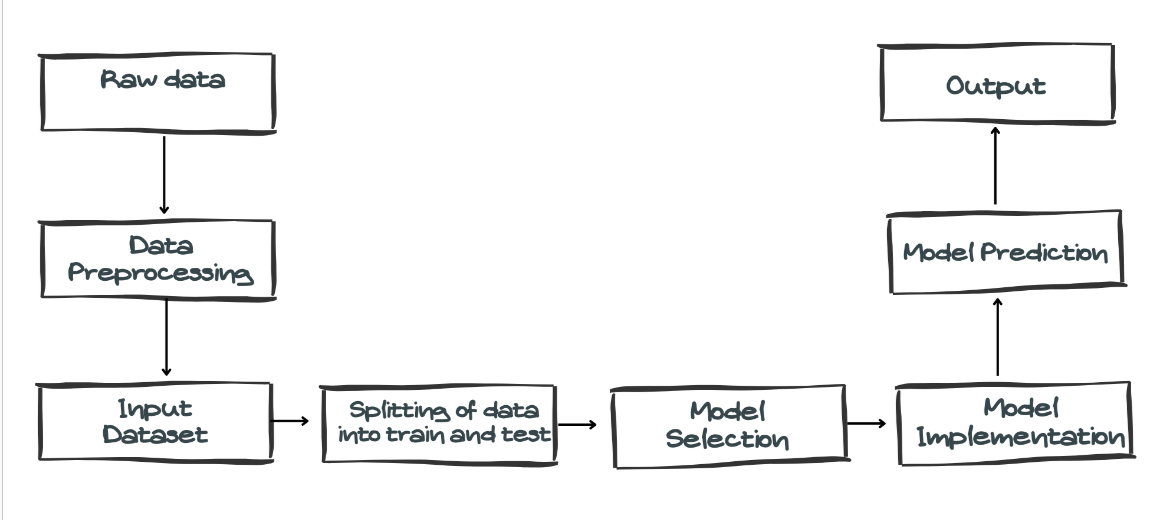
\includegraphics[width=0.5\textwidth]{BLOCK DIAGRAM.png}
    \caption{Workflow of Crop Recommendation Model}
    \label{fig:my_label}
    
\end{figure}

\begin{figure}[h]
    \centering
    \includegraphics[width=0.5\textwidth]{Raw data (4).png}
    \caption{Model Diagram of Crop Recommendation Model}
    \label{fig:my_label}
    
\end{figure}


\subsection{Process Model}

 
%  \caption{Source-pull contours with available input power to the diode set to 6\,dBm.  The impedance is referenced to the junction capacitance of the diode, therefore the lead inductance of the package has been compensated for. Setting $R_{DC}$ to 1080\,$\Omega$ was found to result in the optimal efficiency for this input power.}\label{lpcontours}





 
%  \caption{RF-DC conversion efficiency versus DC load fixed available input powers with 0.6\,dB matching network loss de-embedded.  The maximum efficiency of 72.8\% occurred at 8\,dBm with $R_{DC}$ = 742\,$\Omega$, which is lower than the 1080\,$\Omega$ found during source-pull.  However, the efficiency at 1080\,$\Omega$ is 69.9\% which is very close to the peak value.}\label{final_dc_sweep}


Cross Industry Standard Process for Data Mining, or CRISP DM, is a method that is commonly used and well known in data mining projects. It has six steps: understanding the business, understanding the data, preparing the data, modelling, evaluating, and deploying. The duration of a data mining project is made up of different stages. Figure 3 shows an example of CRISP-DM. The model of CRISP-DM shown in figure 1.

\begin{figure}[h]
    \centering
    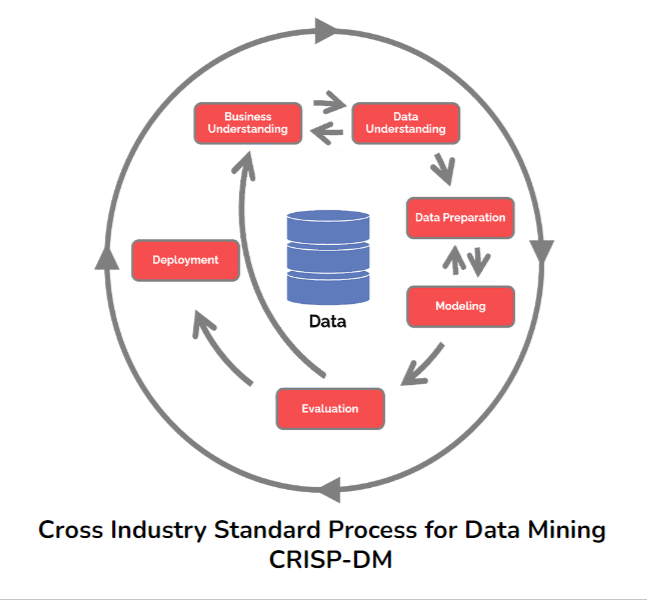
\includegraphics[width=0.5\textwidth]{Crisp Dm.png}
    \caption{Model Diagram of Crop Recommendation Model}
    \label{fig:my_label}
    
\end{figure}
\begin{enumerate}

    \item \textbf{Business Understanding}: During this phase our main focus revolved around comprehending the objectives and requirements of the yield analysis project. The goal was clearly defined; leveraging machine learning techniques to predict and analyze yields. This understanding served as a guiding principle in shaping our approach and ensuring that all activities aligned with our core objectives.
    
    \item \textbf{Data Understanding}: In this stage we collected data. Took the time to familiarize ourselves with it. For our project this involved gathering historical yield information, alongside weather conditions, soil types, and other pertinent variables, which was acquired from Kaggle, which was readily available. This process enabled us to identify any quality issues within the data that could provide insights during the subsequent data preparation phase.
    
    \item \textbf{Data Preparation}: During the process of data preparation we diligently transformed the collected data while taking into account its characteristics. Along the way we encountered instances where certain values were missing or incomplete. To tackle this task we employed imputation techniques to ensure the dataset remained reliable and valuable. Additionally, we transformed attributes such as crop variety into a machine format using data encoding methods.
    
    \item \textbf{Data Modeling}: During the modeling phase we carefully selected machine learning models that were well suited for our data and project objectives. We opted for models like Logistic Regression, KNN, SVM, Decision Tree, and Random Forest as they provide approaches for handling classification and regression tasks. Each model underwent training using the dataset to ensure it learned from the information.
    
    \item \textbf{Data Evaluation}: The evaluation phase played a role in assessing the effectiveness of each model. We utilized metrics such as accuracy, precision, recall, F1 score, ROC AUC curve analysis and examination of confusion matrix to comprehensively evaluate the models. This comprehensive evaluation not only allowed us to determine accuracy but also helped us understand how each model performs in terms of positives/negatives and its ability to handle imbalanced classes.
    
    \item \textbf{Deployment}: In this phase of our project we selected the best performing model based on our evaluation metrics, for deployment. The deployment strategy was tailored to integrate with existing agricultural data management systems.
\end{enumerate}



















% === IV. DATA PREPARATION========================================
% =================================================================================

\subsection{Data Exploration}

In the exploration of the yield analysis, various estimates were calculated for key agricultural parameters. Descriptive statistics were determined for N, P, K, temperature, humidity, pH, and precipitation, including mean, standard deviation, first, second, and third quartile, sample count , minimum and maximum values.The dataset includes samples representing different crops, such as rice, each with specific nutrient levels and environmental conditions, and this analysis provides a quantitative understanding of the factors mean trends and changes in the dataset, which are necessary to determine the development of an effective crop recommendation system . 


\begin{figure}[h]
    \centering
    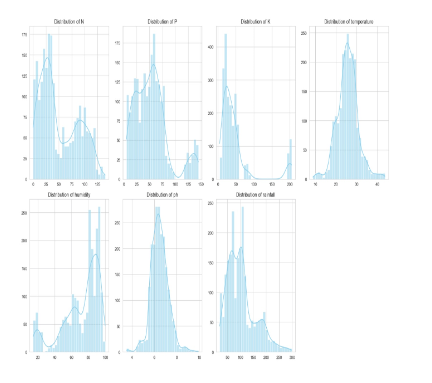
\includegraphics[width=0.5\textwidth]{visual 1.png}
    \caption{Distribution of each feature}
    \label{fig:my_label}
    
\end{figure}


\begin{figure}[h]
    \centering
    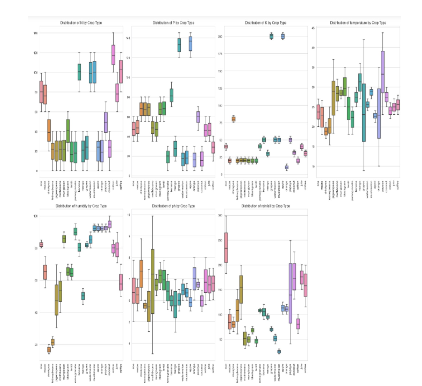
\includegraphics[width=0.5\textwidth]{visual 2.png}
    \caption{Distribution of data by each crop type for each feature}
    \label{fig:my_label}
    
\end{figure}

\begin{figure}[h]
    \centering
    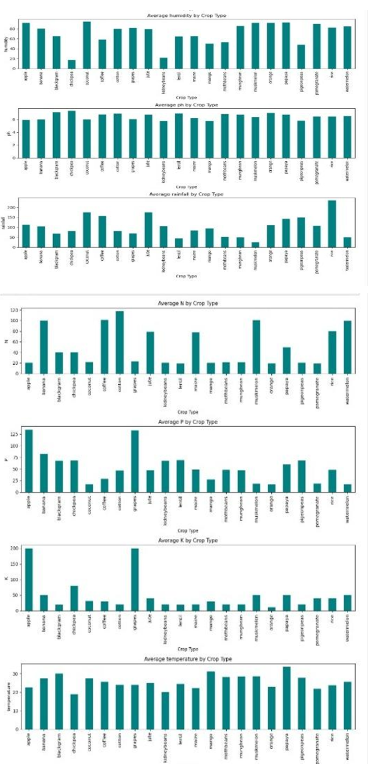
\includegraphics[width=0.5\textwidth]{visual 3.png}
    \caption{Relationship of crops distribution with specific feature
}
    \label{fig:my_label}
    
\end{figure}

\subsection {Data Pre-processing}



Data preprocessing is an important step in developing yield analysis. The data set incorporates various agricultural parameters such as N, P, K, temperature, humidity, pH, rainfall, and corresponding crop indexes. The preprocessing steps required numerical normalization, ensuring that the values were comparable and supported the model accurately. In addition, hierarchical coding was used to convert the crop labels into numerical values suitable for machine learning algorithms. To ensure the completeness of the dataset, imputation techniques were used to deal with missing values. Together, these preprocessing steps improve the quality of the dataset, making it suitable for training and testing machine learning models aimed at accurate and reliable crop recommendations based on agricultural considerations provided.

\subsection {Data Transformation}
During the data transformation stage of the crop recommendation process, segmented crop labels are input and numerical attributes are filled in according to a common scale, which facilitates comprehension of algorithms. Outlier detection strengthens the robustness of the model, while feature engineering and data loss raise relevance. Performance analysis is made easier by dividing the dataset into training and testing sets, and feature redundancy can be found and fixed with the aid of correlation analysis. Normalization is the foundation for efficient model training and guarantees the homogeneity of feature effects. This programming method optimizes the dataset for precise and trustworthy crop recommendations using Python and libraries like scikit-learn and pandas. Figure 7 displays the first few records from the original dataset as shown below. Figure 8 shows the first few normalized records.

\begin{figure}[h]
    \centering
    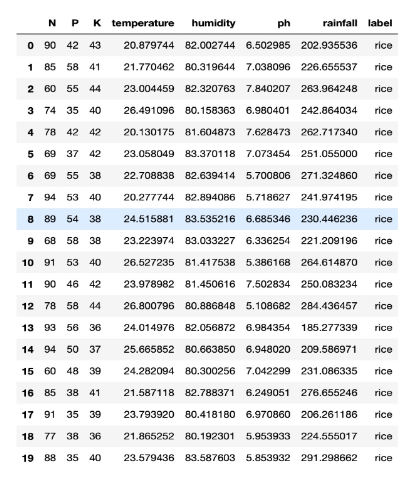
\includegraphics[width=0.5\textwidth]{visual 4.png}
    \caption{First few records from the original dataset}
    \label{fig:my_label}
    
\end{figure}

\begin{figure}[h]
    \centering
    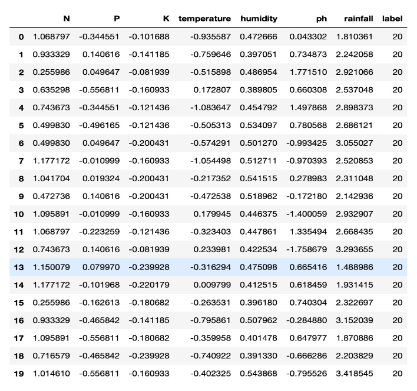
\includegraphics[width=0.5\textwidth]{visual 5.png}
    \caption{First few normalized and encoded records displayed in the above table}
    \label{fig:my_label}
    
\end{figure}

\subsection{Data Encoding}
Data encoding plays an important role in preparing information for machine learning models. Specifically, to transform categorical data in statistics, label coding is applied on the ‘Label’ column representing crop characteristics. This computational representation facilitates the algorithm’s understanding of crop species during training and prediction. This encoding using libraries such as scikit-learn in Python ensures that the machine learning model can correctly interpret and manipulate segmented information, so that this becomes a valuable resource to implement and refine such encoding techniques to enhance the overall performance of recommendation systems.
% 






% ===================================================================================================================================
% ===================================================================================================================================


% An example of a floating figure using the graphicx package.
% Note that \label must occur AFTER (or within) \caption.
% For figures, \caption should occur after the \includegraphics.
% Note that IEEEtran v1.7 and later has special internal code that
% is designed to preserve the operation of \label within \caption
% even when the captionsoff option is in effect. However, because
% of issues like this, it may be the safest practice to put all your
% \label just after \caption rather than within \caption{}.
%
% Reminder: the "draftcls" or "draftclsnofoot", not "draft", class
% option should be used if it is desired that the figures are to be
% displayed while in draft mode.
%
%\begin{figure}[!t]
%\centering
%\includegraphics[width=2.5in]{myfigure}
% where an .eps filename suffix will be assumed under latex, 
% and a .pdf suffix will be assumed for pdflatex; or what has been declared
% via \DeclareGraphicsExtensions.
%\caption{Simulation Results}
%\label{fig_sim}
%\end{figure}

% Note that IEEE typically puts floats only at the top, even when this
% results in a large percentage of a column being occupied by floats.


% An example of a double column floating figure using two subfigures.
% (The subfig.sty package must be loaded for this to work.)
% The subfigure \label commands are set within each subfloat command, the
% \label for the overall figure must come after \caption.
% \hfil must be used as a separator to get equal spacing.
% The subfigure.sty package works much the same way, except \subfigure is
% used instead of \subfloat.
%
%\begin{figure*}[!t]
%\centerline{\subfloat[Case I]\includegraphics[width=2.5in]{subfigcase1}%
%\label{fig_first_case}}
%\hfil
%\subfloat[Case II]{\includegraphics[width=2.5in]{subfigcase2}%
%\label{fig_second_case}}}
%\caption{Simulation results}
%\label{fig_sim}
%\end{figure*}
%
% Note that often IEEE papers with subfigures do not employ subfigure
% captions (using the optional argument to \subfloat), but instead will
% reference/describe all of them (a), (b), etc., within the main caption.


% An example of a floating table. Note that, for IEEE style tables, the 
% \caption command should come BEFORE the table. Table text will default to
% \footnotesize as IEEE normally uses this smaller font for tables.
% The \label must come after \caption as always.
%
%\begin{table}[!t]
%% increase table row spacing, adjust to taste
%\renewcommand{\arraystretch}{1.3}
% if using array.sty, it might be a good idea to tweak the value of
% \extrarowheight as needed to properly center the text within the cells
%\caption{An Example of a Table}
%\label{table_example}
%\centering
%% Some packages, such as MDW tools, offer better commands for making tables
%% than the plain LaTeX2e tabular which is used here.
%\begin{tabular}{|c||c|}
%\hline
%One & Two\\
%\hline
%Three & Four\\
%\hline
%\end{tabular}
%\end{table}


% Note that IEEE does not put floats in the very first column - or typically
% anywhere on the first page for that matter. Also, in-text middle ("here")
% positioning is not used. Most IEEE journals use top floats exclusively.
% Note that, LaTeX2e, unlike IEEE journals, places footnotes above bottom
% floats. This can be corrected via the \fnbelowfloat command of the
% stfloats package.



\section{MODELING}
\begin{figure}[h]
    \centering
    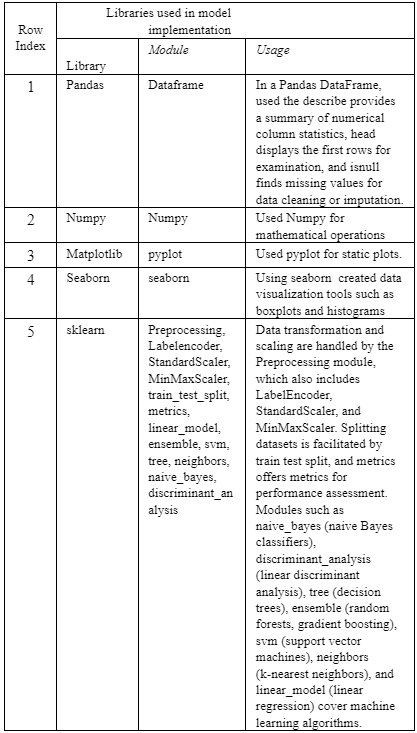
\includegraphics[width=0.5\textwidth]{Screenshot 2023-12-11 020534.png}
    \caption{Libraries used in model implementation}
    \label{fig:my_label}

\end{figure}

In this project,  a number of different machine learning models to reach the goal.Then tested logistic regression, the first linear classification method we looked at, to see how well it worked. Next, used both the Random Forest Classifier and the Decision Tree Classifier to look into the possibilities of ensemble approaches. Support Vector Machine (SVM) was also put into action to show that it could handle decision limits that were not simple. K-Nearest Neighbours (KNN) was used because it was easy to use and good at classifying things. Its performance was better by changing its hyperparameters. The probabilistic method of Gaussian Naive Bayes was also used, and it was tweaked to get better results. Last but not least, linear discriminant analysis (LDA) was put in place. Hyperparameter tuning was used to make each model work even better after it was put in place. In-depth tests were done on the accuracy and other factors of each model. This gave us a clear picture of their pros and cons in terms of our project's goals.

\subsection{Logistic Regression}
A Logistic Regression model is built using the normalised training set of data. When estimates are made on the testing set, accuracy is found. There is also a full evaluation with the calculation of performance measures such as F1 Score, recall, and precision. The model's ability to tell the difference between classes is checked using the Receiver Operating Characteristic Area Under the Curve (ROC-AUC) measure. The printed measures show how well the model categorises, which makes it easier to understand and make decisions.
\subsection{Random Forest}
Random Forest Classifier shows a two-step process. At first, a baseline model is trained to a certain level of accuracy using the default hyperparameters. Then, GridSearchCV is used to tune hyperparameters, which means looking at different values for things like the number of estimators, the maximum depth, the minimum samples split, and the minimum samples leaf. Then, the best hyperparameters found during this hyperparameter tuning process are used to build a Random Forest Classifier that is tuned. Some of the performance measures that are carefully looked at after predictions are made on the testing set are accuracy, precision, recall, the F1 Score, and the Receiver Operating Characteristic Area Under the Curve (ROC-AUC).
\subsection{Decision tree}
The code's first step is to make a Decision Tree Classifier, train it on an 80\% training dataset, and then use a 20\% testing dataset to see how well it did. Next, GridSearchCV is used to do a hyperparameter tuning process. This checks out different mixes of criteria for node splitting, maximum tree depth, and minimum sample needs. After this search, the best hyperparameters are identified and used to build a new Decision Tree model that is learned with the training dataset. The testing sample is used to check how accurate this optimised model is. Along with the calculation of performance measures like F1 Score, recall, and precision, a full evaluation is also given.

\subsection{Support vector machine}
Making a Support Vector Machine (SVM) Classifier and making it work better. First, a basic support vector machine (SVM) model is made, but the hyperparameters are not given outright. It learns from 80\% of the normalised data and is tested on a 20\% test sample to see how well it works. The next step is to tune the hyperparameters by trying out different mixes of gamma values, kernel type (linear, radial basis function, or polynomial), and regularisation parameter C. The best hyperparameters found by the grid search are then used to build an optimised SVM model. This model has been fine-tuned to provide a complete way to create and improve SVM models for better prediction performance. The training dataset is used to teach it, and the testing dataset is used to test how well it learned.
\subsection{K-Nearest Neighbors}
First, a basic KNN model is created without any hyperparameters being given directly. It learns from 80\% of the normalised data and is tested on a 20\% test sample to see how well it works. Then, GridSearchCV is used to fine-tune the hyperparameters by trying out different mixes of the number of neighbours (n neighbors), the weighting method (weights), and the distance metric (p). The best hyperparameters found by the grid search are then used to build an optimised KNN model. This model has been fine-tuned and now provides a complete way to create and improve KNN models for better prediction. The training dataset is used to teach it, and the testing dataset is used to test how well it learned.


\subsection{Linear Discriminant Analysis}

The dataset is first separated into training and testing sets (eighty percent training and twenty percent testing). the information is split into two sets: a training set with 80\% of it being training data and a testing set with 20\% of it being testing data. Then, the training set of data is used to teach the basic LDA model, and the testing set of data is used to check its accuracy and make predictions. Then, GridSearchCV is used to carefully look into different sets of hyperparameters by adding cross-validation—in this case, a 5-fold cross-validation. The best hyperparameters are found by seeing how well they work at different folds. When the determined hyperparameters are added, the optimised LDA model is trained on the whole training dataset, and the testing dataset is used to check how accurate it is. Cross-validated hyperparameter change makes this method a strong way to judge how well the model works.





\section{IMPLEMENTATION}
 For this project, Machine learning models are being used to figure out what kind of crop will work best for this project. The info is put in the Amazon S3 bucket and taken out of it. Because it is so good at many things, Python was chosen as the computer language for this project. That which is being used is Python 3.11.5. The best option is this one because it lets you use a lot of libraries for machine learning models. You can use Collab Notebook and Jupyter Notebook on a local workstation with 16GB RAM and 8 core CPUs to set up, train, confirm, test, and see the different metrics of the models. The tools that were used to build the models are shown in Figure 9.

 






 \section{Evaluation Methods}
 \subsection{Accuracy}
 Accuracy indicates the overall correctness of a classification model. By displaying the ratio of correctly predicted instances to the total number of instances. It offers a thorough evaluation of the model's capacity for accurate prediction across all classes. The accuracy formula is shown in equation 1.


 \begin{figure}[h]
    \centering
    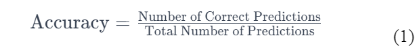
\includegraphics[width=0.3\textwidth]{Screenshot 2023-12-11 010842.png}
\end{figure}

 \subsection{Precision}
 The accuracy of positive predictions is the primary focus of precision. It determines the percentage of actual positive forecasts among all positive predictions. When there is a large cost associated with false positives and it is necessary to reduce the number of falsely detected positive cases, precision becomes especially important. The precision formula is shown in equation2.
 \begin{figure}[h]
    \centering
    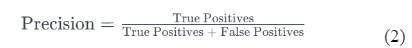
\includegraphics[width=0.3\textwidth]{Screenshot 2023-12-11 010914.png}
   
\end{figure}
 \subsection{Recall}
 Recall measures the model's capacity to recognize all relevant instances among the real positive instances; it is often referred to as sensitivity or true positive rate. Capturing all positive cases is especially important when the cost of false negatives is significant.The formula for Recall is shown in equation3.

 
  \begin{figure}[h]
    \centering
    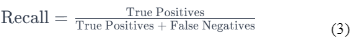
\includegraphics[width=0.3\textwidth]{Recall.png}
\end{figure}


 \subsection{F1 Score}
 The F1 Score is a balanced metric that takes into account both false positives and false negatives. It is calculated as the harmonic mean of precision and recall. It is particularly helpful when a thorough evaluation of the model's performance is required, and it is necessary to find a balance between recall and precision. The formula for F1 Score is shown in equation4.
 \begin{figure}[h]
    \centering
    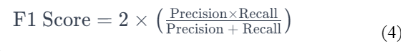
\includegraphics[width=0.3\textwidth]{Screenshot 2023-12-11 020322.png}
\end{figure}
 
\subsection{ROC}
The performance of a binary classification model across various classification thresholds is depicted graphically by the Receiver Operating Characteristic (ROC). The True Positive Rate (Sensitivity) is plotted against the False Positive Rate at different threshold values to form the ROC curve. The equation for ROC is represented in equation5.

\begin{figure}[h]
    \centering
    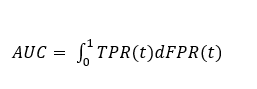
\includegraphics[width=0.2\textwidth]{Screenshot (195).png}
   
\end{figure}

 A classification model's overall performance is measured by the ROC value, often known as the Area Under the ROC Curve (ROC-AUC). Its value ranges from 0 to 1, signifying the area under the ROC curve. Greater capacity of the model to distinguish between positive and negative examples is shown by a higher ROC-AUC value. 





\begin{figure}[h]
    \centering
    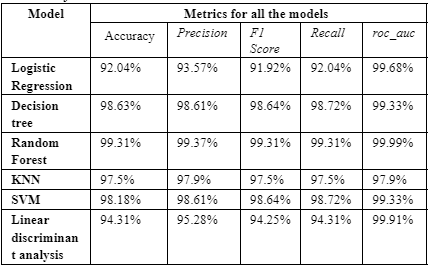
\includegraphics[width=0.4\textwidth]{visual 8.png}
    \caption{Metrics of all the models}
    \label{fig:my_label}

\end{figure}


\section{Deployment}


%Dr. Reveryrand would like to acknowledge the funding by XLIM, Limoges, France. 
Using Python's pickle module, we serialized the Random Forest algorithm that we had trained as a crucial step in developing our crop recommendation system. Through this procedure, we were able to package the model's state,which comprises all parameters and learnt structures into a file that is conveniently loadable and used by our web application framework. The Random Forest model is made up of multiple decision trees that collaborate to produce the best crop recommendation depending on input variables like soil nutrient content and environmental circumstances. It was selected for its resilience and accuracy in handling the multivariate dataset.Through serialization, we were able to maintain the predictive power of the model while also improving system efficiency by removing the requirement for the model to be retrained for every user query, allowing recommendations to be made in real time.

Flask serves as a bridge between the user and our machine learning backend, making it easier to deploy the model into a production environment. Because of its modular and lightweight architecture, Flask was the best option for our system because it allowed for a scalable and maintained codebase. The Flask server deserializes the model and applies it to the input data to forecast an ideal crop after obtaining input data via an intuitive form. The user is then presented with this projection, giving them practical insights unique to their own farming circumstances.The goal of the deployment phase was to minimize the barrier to entry for users with less technical experience by making the application's interface as intuitive as feasible. With the implementation of the crop recommendation system, farmers will be able to make well-informed decisions supported by machine learning insights, marking a significant advancement in the integration of advanced data analytics into agricultural practices.

 \begin{figure}[h]
    \centering
    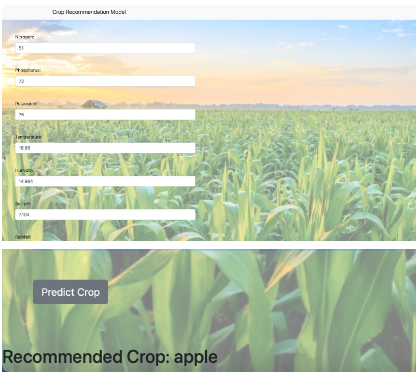
\includegraphics[width=0.4\textwidth]{visual 6.png}
    \caption{Flask implementation}
    \label{fig:my_label}

\end{figure}

\section{IMPACT AFTER RESOLVING PROPOSED PROBLEM}
Our crop recommender system's implementation is a noteworthy development at the nexus of technology and agriculture, and it has the potential to have a substantial impact on sustainable farming methods. The technique reduces the common problem of agricultural mismanagement and promotes more effective use of resources by precisely forecasting the most viable crops for production based on specific soil and environmental conditions. In addition to increasing yields, this optimization maintains biodiversity, lowers the need for chemical fertilizers, and matches crop choices to the land's natural appropriateness. Therefore, the use of our approach might spark a change in farming practices toward more ecologically friendly ones, which is crucial given the issues of climate change and food security.

Moreover, it is important to recognize the crop recommender system's economic impact. The capacity to optimize production potential directly correlates with greater income and livelihood security for smallholder farmers. This tool is a vital advisor in areas where access to agronomic knowledge is limited. It democratizes knowledge that was previously reserved for agricultural professionals. We expect increased crop success rates to strengthen community resilience against food shortages and market volatility as the system gathers traction. Long-term, the worldwide adoption of data-driven crop suggestions may encourage agricultural practice innovation and result in a more resilient and adaptable food production ecosystem.

\section{RESULTS}
To sum up, the assessment of different machine learning models exposes their unique advantages and functionalities. Out of all the models, Random Forest performs the best, with amazing ROC-AUC of 99.99\%, accuracy (99.31\%), and precision (99.37\%). The particular model selected should be determined by the particular needs of the classification task, taking into account the trade-offs between discriminatory power, recall, accuracy, and precision as represented by the ROC-AUC. The Confusion matrix of the Random forest model is represented below in Figure 10.

 \begin{figure}[t]
    \centering
    \includegraphics[width=0.4\textwidth]{visual 7.png}
    \caption{Confusion Matrix for Random Forest Model}
    \label{fig:my_label}

\end{figure}










\section{CONCLUSION}
In conclusion, evaluating several machine learning models reveals their distinct benefits and features. With an astounding ROC-AUC of 99.99\%, accuracy of 99.31\%, recall 99.31\%, and precision of 99.37\%, Random Forest model performs better than all other models.
\section{LIMITATIONS AND FUTURE SCOPE}
Crop recommendation systems are constrained by problems with data quality, a narrow feature scope, regional variability, challenges in accounting for intricate farming practices, and difficulties in embracing new technologies and environments.

Several model groups and the investigation of sophisticated deep learning models are suggested as ways to enhance the accuracy of the crop recommendation process. To provide a thorough analysis, a variety of data types—such as weather, soil, satellite imagery, and historical data—are combined.

% if have a single appendix:
%\appendix[Proof of the Zonklar Equations]
% or
%\appendix  % for no appendix heading
% do not use \section anymore after \appendix, only \section*
% is possibly needed

% use appendices with more than one appendix
% then use \section to start each appendix
% you must declare a \section before using any
% \subsection or using \label (\appendices by itself
% starts a section numbered zero.)
%

% ============================================
%\appendices
%\section{Proof of the First Zonklar Equation}
%Appendix one text goes here %\cite{Roberg2010}.

% you can choose not to have a title for an appendix
% if you want by leaving the argument blank
%\section{}
%Appendix two text goes here.


% use section* for acknowledgement
%\section*{Acknowledgment}


%The authors would like to thank D. Root for the loan of the SWAP. The SWAP that can ONLY be usefull in Boulder...


% Can use something like this to put references on a page
% by themselves when using endfloat and the captionsoff option.
\ifCLASSOPTIONcaptionsoff
  \newpage
\fi



% trigger a \newpage just before the given reference
% number - used to balance the columns on the last page
% adjust value as needed - may need to be readjusted if
% the document is modified later
%\IEEEtriggeratref{8}
% The "triggered" command can be changed if desired:
%\IEEEtriggercmd{\enlargethispage{-5in}}

% ====== REFERENCE SECTION

%\begin{thebibliography}{1}

% IEEEabrv,



%\end{thebibliography}
% biography section
% 
% If you have an EPS/PDF photo (graphicx package needed) extra braces are
% needed around the contents of the optional argument to biography to prevent
% the LaTeX parser from getting confused when it sees the complicated
% \includegraphics command within an optional argument. (You could create
% your own custom macro containing the \includegraphics command to make things
% simpler here.)
%\begin{biography}[{\includegraphics[width=1in,height=1.25in,clip,keepaspectratio]{mshell}}]{Michael Shell}
% or if you just want to reserve a space for a photo:

% ==== SWITCH OFF the BIO for submission
% ==== SWITCH OFF the BIO for submission


\begin{thebibliography}{99}

\bibitem{b1} B. S. Sri, G. Pavani, B. Y. S. Sindhuja, V. Swapna and P. L. Priyanka, "An Improved Machine Learning based Crop Recommendation System," 2023 International Conference on Sustainable Computing and Data Communication Systems (ICSCDS), Erode, India, 2023, pp. 64-68, doi: 10.1109/ICSCDS56580.2023.10105119.

\bibitem{b2} D. Modi, A. V. Sutagundar, V. Yalavigi and A. Aravatagimath, "Crop Recommendation Using Machine Learning Algorithm," 2021 5th International Conference on Information Systems and Computer Networks (ISCON), Mathura, India, 2021, pp. 1-5, doi: 10.1109/ISCON52037.2021.9702392.

\bibitem{b3}S. Vaishnavi., M. Shobana., R. Sabitha. and S. Karthik., "Agricultural Crop Recommendations based on Productivity and Season," 2021 7th International Conference on Advanced Computing and Communication Systems (ICACCS), Coimbatore, India, 2021, pp. 883-886, doi: 10.1109/ICACCS51430.2021.9441736.
\bibitem{b4}T. van Klompenburg, A. Kassahun, and C. Catal, "Crop yield prediction using machine learning: A systematic literature review," Computers and Electronics in Agriculture, vol. 177, 2020, article 105709, ISSN 0168-1699, doi: 10.1016/j.compag.2020.105709.
\bibitem{b5}Paola Battilani, Amedeo Pietri, Carlo Barbano, Andrea Scandolara, Terenzio Bertuzzi, and Adriano Marocco, “Logistic Regression Modeling of Cropping Systems To Predict Fumonisin Contamination in Maize”, Journal of Agricultural and Food Chemistry 2008 56 (21), 10433-10438, DOI: 10.1021/jf801809d.
\bibitem{b6}N. H. Kulkarni, G. N. Srinivasan, B. M. Sagar and N. K. Cauvery, "Improving Crop Productivity Through A Crop Recommendation System Using Ensembling Technique," 2018 3rd International Conference on Computational Systems and Information Technology for Sustainable Solutions (CSITSS), Bengaluru, India, 2018, pp. 114-119, doi: 10.1109/CSITSS.2018.8768790.
\bibitem{b7}J. Chopda, H. Raveshiya, S. Nakum and V. Nakrani, "Cotton Crop Disease Detection using Decision Tree Classifier," 2018 International Conference on Smart City and Emerging Technology (ICSCET), Mumbai, India, 2018, pp. 1-5, doi: 10.1109/ICSCET.2018.8537336.
\bibitem{b8}T. K. Mishra, S. K. Mishra, K. J. Sai, B. S. Alekhya and A. R. Nishith, "Crop Recommendation System using KNN and Random Forest considering Indian Data set," 2021 19th OITS International Conference on Information Technology (OCIT), Bhubaneswar, India, 2021, pp. 308-312, doi: 10.1109/OCIT53463.2021.00068.
\bibitem{b9}N. Gandhi, L. J. Armstrong, O. Petkar and A. K. Tripathy, "Rice crop yield prediction in India using support vector machines," 2016 13th International Joint Conference on Computer Science and Software Engineering (JCSSE), Khon Kaen, Thailand, 2016, pp. 1-5, doi: 10.1109/JCSSE.2016.7748856.
\bibitem{b10}A. Suresh, P. Ganesh Kumar and M. Ramalatha, "Prediction of major crop yields of Tamilnadu using K-means and Modified KNN," 2018 3rd International Conference on Communication and Electronics Systems (ICCES), Coimbatore, India, 2018, pp. 88-93, doi: 10.1109/CESYS.2018.8723956.
\bibitem{b11}Deepika C, Gnanamalar R P, Thangaraj K, Revathy N, Karthikeyan A, “Linear discriminant analysis of grain quality traits in rice (Oryza sativa L.) using the digital imaging technique”, Journal of Cereal Science, Volume 109, 2023, 103609, ISSN 0733-5210.  https://doi.org/10.1016/j.jcs.2022.103609


\end{thebibliography}


%----------- Online courses-----------

\section{Drive Link}
\url{https://drive.google.com/drive/folders/1HxlNgBJ_Nd-begwUxrTsOIEhms-rg-d8?usp=sharing}

\section{Youtube Link}
\url{https://www.youtube.com/watch?v=5kGN65bF_N8}

\section{Github Link}
\url{https://github.com/swarajkul/DATA-245}


%% if you will not have a photo at all:
%\begin{IEEEbiographynophoto}{Ignacio Ramos}
%(S'12) received the B.S. degree in electrical engineering from the University of Illinois at Chicago in 2009, and is currently working toward the Ph.D. degree at the University of Colorado at Boulder. From 2009 to 2011, he was with the Power and Electronic Systems Department at Raytheon IDS, Sudbury, MA. His research interests include high-efficiency microwave power amplifiers, microwave DC/DC converters, radar systems, and wireless power transmission.
%\end{IEEEbiographynophoto}

%% insert where needed to balance the two columns on the last page with
%% biographies
%%\newpage

%\begin{IEEEbiographynophoto}{Jane Doe}
%Biography text here.
%\end{IEEEbiographynophoto}
% ==== SWITCH OFF the BIO for submission
% ==== SWITCH OFF the BIO for submission



% You can push biographies down or up by placing
% a \vfill before or after them. The appropriate
% use of \vfill depends on what kind of text is
% on the last page and whether or not the columns
% are being equalized.

\vfill

% Can be used to pull up biographies so that the bottom of the last one
% is flush with the other column.
%\enlargethispage{-5in}



% that's all folks
\end{document}


